\documentclass[10pt]{article}\usepackage[]{graphicx}\usepackage[]{xcolor}
% maxwidth is the original width if it is less than linewidth
% otherwise use linewidth (to make sure the graphics do not exceed the margin)
\makeatletter
\def\maxwidth{ %
  \ifdim\Gin@nat@width>\linewidth
    \linewidth
  \else
    \Gin@nat@width
  \fi
}
\makeatother

\definecolor{fgcolor}{rgb}{0.345, 0.345, 0.345}
\newcommand{\hlnum}[1]{\textcolor[rgb]{0.686,0.059,0.569}{#1}}%
\newcommand{\hlstr}[1]{\textcolor[rgb]{0.192,0.494,0.8}{#1}}%
\newcommand{\hlcom}[1]{\textcolor[rgb]{0.678,0.584,0.686}{\textit{#1}}}%
\newcommand{\hlopt}[1]{\textcolor[rgb]{0,0,0}{#1}}%
\newcommand{\hlstd}[1]{\textcolor[rgb]{0.345,0.345,0.345}{#1}}%
\newcommand{\hlkwa}[1]{\textcolor[rgb]{0.161,0.373,0.58}{\textbf{#1}}}%
\newcommand{\hlkwb}[1]{\textcolor[rgb]{0.69,0.353,0.396}{#1}}%
\newcommand{\hlkwc}[1]{\textcolor[rgb]{0.333,0.667,0.333}{#1}}%
\newcommand{\hlkwd}[1]{\textcolor[rgb]{0.737,0.353,0.396}{\textbf{#1}}}%
\let\hlipl\hlkwb

\usepackage{framed}
\makeatletter
\newenvironment{kframe}{%
 \def\at@end@of@kframe{}%
 \ifinner\ifhmode%
  \def\at@end@of@kframe{\end{minipage}}%
  \begin{minipage}{\columnwidth}%
 \fi\fi%
 \def\FrameCommand##1{\hskip\@totalleftmargin \hskip-\fboxsep
 \colorbox{shadecolor}{##1}\hskip-\fboxsep
     % There is no \\@totalrightmargin, so:
     \hskip-\linewidth \hskip-\@totalleftmargin \hskip\columnwidth}%
 \MakeFramed {\advance\hsize-\width
   \@totalleftmargin\z@ \linewidth\hsize
   \@setminipage}}%
 {\par\unskip\endMakeFramed%
 \at@end@of@kframe}
\makeatother

\definecolor{shadecolor}{rgb}{.97, .97, .97}
\definecolor{messagecolor}{rgb}{0, 0, 0}
\definecolor{warningcolor}{rgb}{1, 0, 1}
\definecolor{errorcolor}{rgb}{1, 0, 0}
\newenvironment{knitrout}{}{} % an empty environment to be redefined in TeX

\usepackage{alltt}
\usepackage[utf8]{inputenc}
\usepackage[spanish]{babel}
\usepackage[letterpaper, margin=1.5in, headheight=16pt]{geometry}
\usepackage{mathtools}
\usepackage{amsfonts}
\usepackage{amsmath}
\usepackage{amssymb}
\usepackage{amsthm}
\usepackage{graphicx}
\usepackage{enumitem}
\usepackage{caption}
\usepackage{subcaption}
\usepackage{titling}
\usepackage{float}
\usepackage{xcolor}
\usepackage{hyperref}
\definecolor{cimatred}{RGB}{122,51,69}
\hypersetup{
    colorlinks=true,
    linkcolor=cimatred,
    filecolor=cimatred,      
    urlcolor=cimatred,
    citecolor=cimatred
}
\urlstyle{same}
\newtheorem{theorem}{Teorema}
\newtheorem{corollary}{Corolario}[theorem]
\newtheorem{lemma}[theorem]{Lema}
\newtheorem{definition}{Definición}
\newtheorem{plain}{Proposición}
\newtheorem*{remark}{Observación}
\spanishdecimal{.}
\newcommand{\N}{\mathbb{N}}
\newcommand{\Z}{\mathbb{Z}}
\newcommand{\Q}{\mathbb{Q}}
\newcommand{\R}{\mathbb{R}}
\newcommand{\C}{\mathbb{C}}
\newcommand{\norm}[1]{\left\|#1\right\|}
\newcommand{\abs}[1]{\left|#1\right|}
\newcommand{\comp}[1]{#1^\mathrm{C}}
\newcommand{\mean}[1]{\mathbb{E}\left[#1\right]}

\renewcommand{\baselinestretch}{1}
\DeclareMathOperator{\indic} {\textup{\large 1}}
\DeclareMathOperator{\Prob} {\mathbb P}
\DeclareMathOperator{\E} {\mathbb E}
\DeclareMathOperator{\V} {\mathbb V}
\DeclareMathOperator{\Normal} {\mathcal{N}}


\usepackage{fixdif}



\author{José Miguel Saavedra Aguilar}
\title{Ayudantía 2}
\IfFileExists{upquote.sty}{\usepackage{upquote}}{}
\begin{document}

\pagestyle{plain}

\setlength{\parskip}{10pt}
\setlength{\parindent}{5pt}
\begin{minipage}{0.2\linewidth}
\vspace{-1cm}

\includegraphics[width=0.9\linewidth]{logoCIMAT11.png}
\end{minipage}
\begin{minipage}{0.7\linewidth}
\vspace{-1cm}
\noindent {\large \color{cimatred}\textbf{Centro de Investigación en Matemáticas, A.C.}}\\
\textbf{Inferencia Estadística}
\end{minipage}
\vspace{-5mm}
\begin{center}
\textbf{\large \thetitle}\\   %TITULO
\vspace{3mm}
\theauthor
\end{center}
\vspace{-5mm}
\rule{\linewidth}{0.1mm}

Esto es un documento creado para ejemplificar el uso de knitr. Es recomendable consultar el libro de Yihui Xie \cite{Xie2015} para mayor información.
\begin{knitrout}
\definecolor{shadecolor}{rgb}{0.969, 0.969, 0.969}\color{fgcolor}\begin{kframe}
\begin{alltt}
\hlkwd{read_chunk}\hlstd{(}\hlstr{'Ayudantia 1.R'}\hlstd{)}
\end{alltt}
\end{kframe}
\end{knitrout}

\section{Ejemplo 1}

Para una v.a. $X\sim \mathrm{exp}$, graficamos la función de densidad para distintas tasas $\lambda = 5, 2, 0.5$.




\begin{knitrout}
\definecolor{shadecolor}{rgb}{0.969, 0.969, 0.969}\color{fgcolor}\begin{kframe}
\begin{alltt}
\hlcom{# Creamos un vector de 100 puntos en el soporte.}
\hlcom{# En nuestro caso, tomamos de 0 a 10.}
\hlstd{x} \hlkwb{<-} \hlkwd{seq}\hlstd{(}\hlnum{0}\hlstd{,} \hlnum{10}\hlstd{,} \hlkwc{length} \hlstd{=} \hlnum{100}\hlstd{)}
\end{alltt}
\end{kframe}
\end{knitrout}

\begin{knitrout}
\definecolor{shadecolor}{rgb}{0.969, 0.969, 0.969}\color{fgcolor}\begin{kframe}
\begin{alltt}
\hlcom{# y es la función de densidad elegida evaluada en los puntos de x}
\hlcom{# Para obtener la función de densidad, se toma "d"+nombre de la distribución, por ejemplo dnorm o dexp}
\hlstd{y1} \hlkwb{<-} \hlkwd{dexp}\hlstd{(x,} \hlkwc{rate} \hlstd{=} \hlnum{5}\hlstd{)}
\hlstd{y2} \hlkwb{<-} \hlkwd{dexp}\hlstd{(x,} \hlkwc{rate} \hlstd{=} \hlnum{0.5}\hlstd{)}
\hlstd{y3} \hlkwb{<-} \hlkwd{dexp}\hlstd{(x,} \hlkwc{rate} \hlstd{=} \hlnum{2}\hlstd{)}
\end{alltt}
\end{kframe}
\end{knitrout}
\begin{knitrout}
\definecolor{shadecolor}{rgb}{0.969, 0.969, 0.969}\color{fgcolor}\begin{figure}[htbp]

{\centering 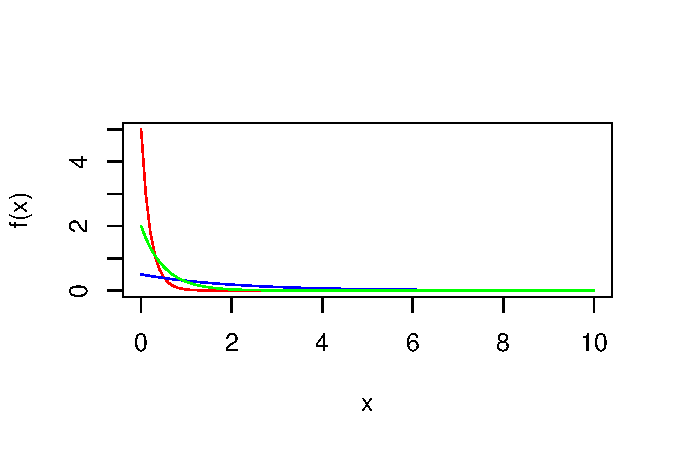
\includegraphics[width=\maxwidth]{figure/densidades-1} 

}

\caption[Densidad de una v.a]{Densidad de una v.a. exponencial para distintas medias}\label{fig:densidades}
\end{figure}

\end{knitrout}
Ahora, graficamos las respectivas funciones de distribución de $X$.

\begin{knitrout}
\definecolor{shadecolor}{rgb}{0.969, 0.969, 0.969}\color{fgcolor}\begin{kframe}
\begin{alltt}
\hlcom{# f es la función de distribución asociada evaluada en los puntos de x}
\hlcom{# Para obtener la función de densidad, se toma}
\hlcom{# "p"+nombre de la distribución, por ejemplo pnorm o pexp}
\hlstd{f1} \hlkwb{<-} \hlkwd{pexp}\hlstd{(x,} \hlkwc{rate} \hlstd{=} \hlnum{5} \hlstd{)}
\hlstd{f2} \hlkwb{<-} \hlkwd{pexp}\hlstd{(x,} \hlkwc{rate} \hlstd{=} \hlnum{0.5} \hlstd{)}
\hlstd{f3} \hlkwb{<-} \hlkwd{pexp}\hlstd{(x,} \hlkwc{rate} \hlstd{=} \hlnum{2} \hlstd{)}
\end{alltt}
\end{kframe}
\end{knitrout}

\begin{knitrout}
\definecolor{shadecolor}{rgb}{0.969, 0.969, 0.969}\color{fgcolor}\begin{figure}[ht]

{\centering 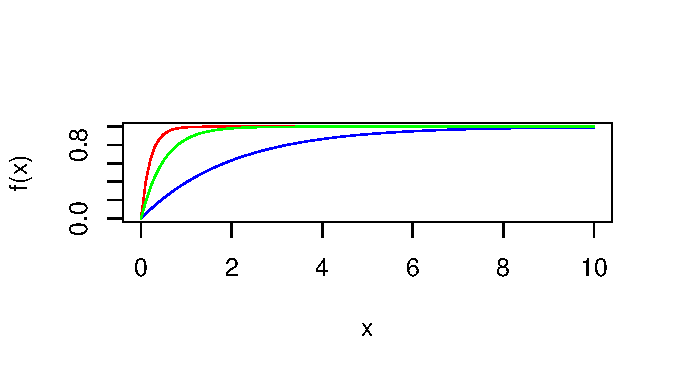
\includegraphics[width=\maxwidth]{figure/distribuciones-1} 

}

\caption[Distribución exponencial para distintas medias]{Distribución exponencial para distintas medias}\label{fig:distribuciones}
\end{figure}

\end{knitrout}


Para $\lambda=0.5$, simulamos una muestra aleatoria de tamaño $n=100$ datos de $X$.

\begin{knitrout}
\definecolor{shadecolor}{rgb}{0.969, 0.969, 0.969}\color{fgcolor}\begin{kframe}
\begin{alltt}
\hlcom{# Tomamos n=100 y simulamos n datos pseudoaleatorios de la distribución elegida}
\hlcom{# Para obtener los datos aleatorios, se toma}
\hlcom{# "r"+nombre de la distribución, por ejemplo rnorm o rexp}
\hlstd{n} \hlkwb{<-} \hlnum{100}
\hlstd{z} \hlkwb{<-} \hlkwd{rexp}\hlstd{(n,}\hlkwc{rate} \hlstd{=} \hlnum{0.5}\hlstd{)}
\end{alltt}
\end{kframe}
\end{knitrout}
\begin{knitrout}
\definecolor{shadecolor}{rgb}{0.969, 0.969, 0.969}\color{fgcolor}\begin{figure}[hb!]

{\centering 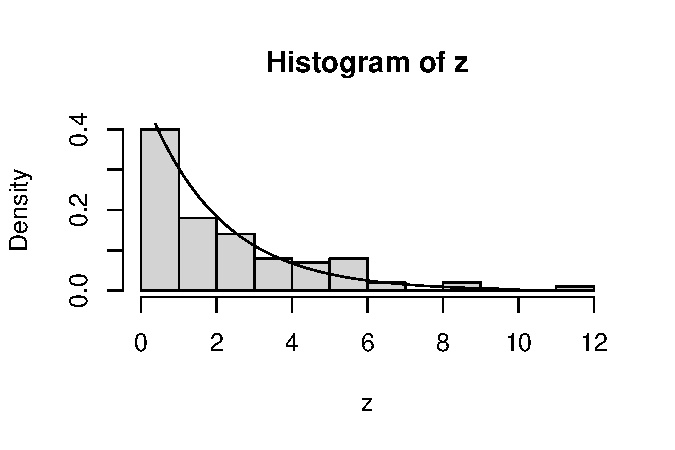
\includegraphics[width=\maxwidth]{figure/histograma-1} 

}

\caption[Histograma de una m.a]{Histograma de una m.a. Exponencial con $\lambda=0.5$}\label{fig:histograma}
\end{figure}

\end{knitrout}
Los datos que simulamos tienen media muestral $2.1625306$ y varianza muestral $4.8139365$.\\
Ordenamos los puntos simulados en $x_{(1)},x_{(2)}, \ldots, x_{(n)}$. Les asociamos $k_i$ definido por
\begin{align}
k_i &= \frac{i}{n+1}
\end{align}

\begin{knitrout}
\definecolor{shadecolor}{rgb}{0.969, 0.969, 0.969}\color{fgcolor}\begin{kframe}
\begin{alltt}
\hlcom{#Ahora vamos a ordenar los datos como indica la tarea.}
\hlstd{z2} \hlkwb{<-} \hlkwd{sort}\hlstd{(z)}
\hlcom{# Inicializamos k =i/n+1}
\hlstd{k} \hlkwb{<-} \hlkwd{numeric}\hlstd{()}

\hlkwa{for} \hlstd{(i} \hlkwa{in} \hlnum{1}\hlopt{:}\hlstd{n) \{}
   \hlstd{k[i]} \hlkwb{<-} \hlstd{i}\hlopt{/}\hlstd{(n}\hlopt{+}\hlnum{1}\hlstd{)}
\hlstd{\}}
\end{alltt}
\end{kframe}
\end{knitrout}
\begin{knitrout}
\definecolor{shadecolor}{rgb}{0.969, 0.969, 0.969}\color{fgcolor}\begin{figure}[ht]

{\centering 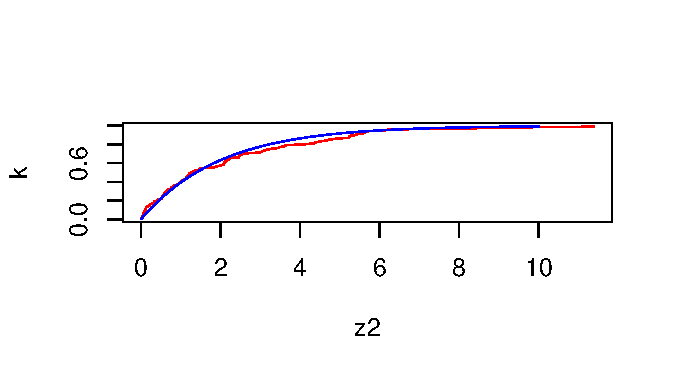
\includegraphics[width=\maxwidth]{figure/FDE-1} 

}

\caption[Comparación entre la función de densidad empírica y la teórica a partir de la muestra]{Comparación entre la función de densidad empírica y la teórica a partir de la muestra}\label{fig:FDE}
\end{figure}

\end{knitrout}
Para conocer más sobre la función de distribución empírica, pueden consultar \href{https://en.wikipedia.org/wiki/Empirical_distribution_function}{Wikipedia}.

\section{Ejemplo 2}
Una variable aleatoria discreta $X$ tiene función de masa de probabilidad:
$$
\begin{array}{cccccc}{x} & {0} & {1} & {2} & {3} & {4} \\ \hline p(x) & {0.1} & {0.2} & {0.2} & {0.2} & {0.3}\end{array}
$$
Utilicen el teorema de la transformación inversa para generar una muestra aleatoria de tamaño 1000 de la distribución de $X$. Construyan una tabla de frecuencias relativas y comparen las probabilidades empíricas con las teóricas.\\
Repitan considerando la función de R sample.
\begin{knitrout}
\definecolor{shadecolor}{rgb}{0.969, 0.969, 0.969}\color{fgcolor}\begin{kframe}
\begin{alltt}
\hlcom{#Ejemplo 2}
\hlkwd{set.seed}\hlstd{(}\hlnum{157017}\hlstd{)}
\hlstd{prob} \hlkwb{<-} \hlkwd{c}\hlstd{(}\hlnum{.1}\hlstd{,}\hlnum{.3}\hlstd{,}\hlnum{.5}\hlstd{,}\hlnum{.7}\hlstd{,}\hlnum{1}\hlstd{)}
\hlstd{frec} \hlkwb{<-} \hlkwd{findInterval}\hlstd{(}\hlkwd{runif}\hlstd{(}\hlnum{1000}\hlstd{),prob)}
\hlkwd{table}\hlstd{(frec)}\hlopt{/}\hlnum{1000}
\end{alltt}
\begin{verbatim}
## frec
##     0     1     2     3     4 
## 0.125 0.168 0.224 0.185 0.298
\end{verbatim}
\begin{alltt}
\hlkwd{set.seed}\hlstd{(}\hlnum{157017}\hlstd{)}
\hlstd{frecSample}\hlkwb{<-}\hlkwd{sample}\hlstd{(}\hlkwc{x}\hlstd{=}\hlnum{0}\hlopt{:}\hlnum{4}\hlstd{,}\hlkwc{size}\hlstd{=}\hlnum{1000}\hlstd{,}\hlkwc{replace} \hlstd{=} \hlnum{TRUE}\hlstd{,}\hlkwc{prob} \hlstd{=} \hlkwd{c}\hlstd{(}\hlnum{0.1}\hlstd{,}\hlnum{0.2}\hlstd{,}\hlnum{0.2}\hlstd{,}\hlnum{0.2}\hlstd{,}\hlnum{0.3}\hlstd{))}
\hlkwd{table}\hlstd{(frecSample)}\hlopt{/}\hlnum{1000}
\end{alltt}
\begin{verbatim}
## frecSample
##     0     1     2     3     4 
## 0.103 0.195 0.224 0.185 0.293
\end{verbatim}
\end{kframe}
\end{knitrout}

\section{Ejemplo 3}
Obtengan una muestra de $10,000$ números de la siguiente distribución discreta:
$$
p(x)=\frac{2 x}{k(k+1)}, x=1,2, \ldots, k
$$
para $k=100$
\begin{knitrout}
\definecolor{shadecolor}{rgb}{0.969, 0.969, 0.969}\color{fgcolor}\begin{kframe}
\begin{alltt}
\hlcom{#Ejemplo 3}
\hlstd{p}\hlkwb{<-}\hlkwa{function}\hlstd{(}\hlkwc{n}\hlstd{)\{}
  \hlstd{values}\hlkwb{=}\hlkwd{sample}\hlstd{(}\hlnum{1}\hlopt{:}\hlnum{100}\hlstd{,n,}\hlkwc{replace}\hlstd{=T)}
  \hlstd{prob}\hlkwb{=}\hlstd{(}\hlnum{2}\hlopt{*}\hlstd{values)}\hlopt{/}\hlstd{(}\hlnum{100}\hlopt{*}\hlnum{101}\hlstd{)}
  \hlkwd{return}\hlstd{(prob)}
\hlstd{\}}
\hlkwd{head}\hlstd{(}\hlkwd{p}\hlstd{(}\hlnum{10000}\hlstd{),}\hlkwc{n}\hlstd{=}\hlnum{30}\hlstd{)}
\end{alltt}
\begin{verbatim}
##  [1] 0.0091089109 0.0172277228 0.0106930693 0.0011881188 0.0112871287
##  [6] 0.0164356436 0.0001980198 0.0065346535 0.0196039604 0.0061386139
## [11] 0.0116831683 0.0108910891 0.0106930693 0.0194059406 0.0077227723
## [16] 0.0108910891 0.0186138614 0.0186138614 0.0182178218 0.0003960396
## [21] 0.0091089109 0.0142574257 0.0166336634 0.0172277228 0.0081188119
## [26] 0.0037623762 0.0011881188 0.0196039604 0.0061386139 0.0150495050
\end{verbatim}
\end{kframe}
\end{knitrout}

\section{Ejemplo 4}
Una compañía de seguros tiene 1000 asegurados, cada uno de los cuales presentará de manera independiente una reclamación en el siguiente mes con probabilidad $p = 0.09245$. Suponiendo que las cantidades de los reclamos hechos son variables aleatorias Gamma(7000,1), hagan simulación para estimar la probabilidad de que la suma de los reclamos exceda $\$ 500,000$.
\begin{knitrout}
\definecolor{shadecolor}{rgb}{0.969, 0.969, 0.969}\color{fgcolor}\begin{kframe}
\begin{alltt}
\hlcom{#Ejemplo 4}
\hlstd{mayor} \hlkwb{<-} \hlnum{0}
\hlkwa{for}\hlstd{(i} \hlkwa{in} \hlnum{1}\hlopt{:}\hlnum{10000}\hlstd{)\{}
  \hlstd{reclammaciones}\hlkwb{<-}\hlkwd{sum}\hlstd{(}\hlkwd{rbinom}\hlstd{(}\hlnum{1000}\hlstd{,} \hlnum{1}\hlstd{,} \hlnum{0.09245}\hlstd{))}
  \hlstd{montos} \hlkwb{<-} \hlkwd{sum}\hlstd{(}\hlkwd{rgamma}\hlstd{(reclammaciones,} \hlnum{7000}\hlstd{,} \hlnum{1}\hlstd{))}
  \hlkwa{if}\hlstd{(montos} \hlopt{>} \hlnum{500000}\hlstd{)\{}
    \hlstd{mayor}\hlkwb{=} \hlstd{mayor}\hlopt{+}\hlnum{1}
  \hlstd{\}}
\hlstd{\}}
\hlstd{mayor}\hlopt{/}\hlnum{10000}
\end{alltt}
\begin{verbatim}
## [1] 0.9897
\end{verbatim}
\end{kframe}
\end{knitrout}

\bibliography{biblio}
\bibliographystyle{IEEEtranS}
\end{document}
